\documentclass[11pt,reqno]{article}
\usepackage{amsmath,amssymb,mathrsfs,amsthm}
\usepackage[UTF8]{ctex}
%\usepackage{xeCJK}
%\setCJKmainfont{SimSum}

\usepackage{graphicx,cite,cases}
%\usepackage[pagewise]{lineno}\linenumbers
%\usepackage{refcheck}
\usepackage{xcolor}
\usepackage{bm}			% 公式加粗
\usepackage{tabularx}   % 绘制定宽表格
\usepackage{authblk}	% 添加更多作者信息
\usepackage{appendix} 	% 生成附录
\usepackage{listings}   % 附录里的代码, 支持语言高亮
\usepackage{hyperref}   % 超链接, 自动跳转
\usepackage{subfigure}  % 插入多张图片
\usepackage{tikz}		% 代码作图


\setlength{\topmargin}{-1.5cm}
\setlength{\oddsidemargin}{0.0cm}
\setlength{\evensidemargin}{0.0cm}
\setlength{\textwidth}{16.7cm}
\setlength{\textheight}{23cm}
\headheight 20pt
\headsep    26pt
\footskip 0.4in

%%%%% 关于公式编号问题 %%%%%
%统一用equation环境
%如果需要加括号用\begin{cases}
%如果公式过长需要分行用\begin{split}
%如果一个equation里面需要多个公式, emmm没研究过

\newtheorem{theorem}{Theorem}[section]
\newtheorem{corollary}[theorem]{Corollary}
\newtheorem{lemma}[theorem]{Lemma}
\newtheorem{proposition}[theorem]{Proposition}
\newtheorem{remark}[theorem]{Remark}
\newtheorem{definition}[theorem]{Definition}
\numberwithin{equation}{section}


\renewcommand{\d}{\,\mathrm d}
\usepackage{algorithm,algorithmicx}  %写伪代码
\usepackage{algpseudocode}			% 写伪代码
%%%%%% 算法部分改为中文显示 %%%%%%%%%
%%\floatname{algorithm}{算法}
\renewcommand{\algorithmicrequire}{\textbf{Input:}}
\renewcommand{\algorithmicensure}{\textbf{Output:}}

%% Ctrl+Alt+R 编译
%% Ctrl+Alt+V 打开文档

\begin{document}

\title{微分方程数值解计算实习Lecture 7}

\author{朱荃凡}
\affil{(吉林大学数学系计算唐班)}
\date{\today}

\maketitle

\vspace{50pt}

\section{问题重述}

如图所示,\ $\Omega$表示$[0,1]^2$的区域,\ $\Gamma_1,\Gamma_2,\Gamma_3,\Gamma_4$
是它的四条边:
\begin{center}
	\begin{tikzpicture}[scale=2.5]
		% 绘制坐标轴
		\draw[->] (-0.2,0) -- (1.3,0) node[below] {$x$};
		\draw[->] (0,-0.2) -- (0,1.3) node[left] {$y$};
		% 绘制坐标轴标签
		\foreach \x in {}
			\draw (\x,0.05) -- (\x,-0.05) node[below] {$\x$};
		\foreach \y in {}
			\draw (0.05,\y) -- (-0.05,\y) node[left] {$\y$};
		% 绘制矩形
		\draw[fill=gray!20] (0,0) rectangle (1,1);
		\node[below left] at (0,0){$O$};
		\node[below] at (1,0){$(1,0)$};
		\node[left] at (0,1){$(0,1)$};
		\node[right] at (1,1){$(1,1)$};
		\node[above right] at (0.4,0.4){$\Omega$};
		\node[left] at (0,0.5){$\Gamma_1$};
		\node[right] at (1,0.5){$\Gamma_2$};
		\node[below] at (0.5,0){$\Gamma_3$};
		\node[above] at (0.5,1){$\Gamma_4$};
	\end{tikzpicture}
\end{center}
利用三角剖分线性元元求解区域$\Omega$区域上的偏微分问题:
\begin{equation}\label{Eqn1}
	\left\{\begin{matrix}
		-\Delta u-2\pi^2u=-2\pi^2xy,&\mathrm{in}\ \Omega,\\
		u(x,y)=0,&\mathrm{in}\ \Gamma_1,\Gamma_3,\\
	   \partial_x u(x,y)=y-\pi\sin(\pi y),&\mathrm{in}\ \Gamma_2,\\
	   \partial_y u(x,y)=x-\pi\sin(\pi x),&\mathrm{in}\ \Gamma_4.
	   \end{matrix}\right.
\end{equation}
其相应的的真解为
\begin{equation}
	u^*=xy+\sin(\pi x)\sin(\pi y).
\end{equation}

\newpage


\section{程序结果}

相较于上次Lagrange双线元的程序, 这次仅在生成刚度矩阵和右端项上有所区别,但原理类似,
因此不再赘述.

\subsection{数值解图像}
这里展示了剖分数$N=10$时的数值解和真解图像(画真解图像也是要剖分的).
\begin{figure}[h]
	\centering
	  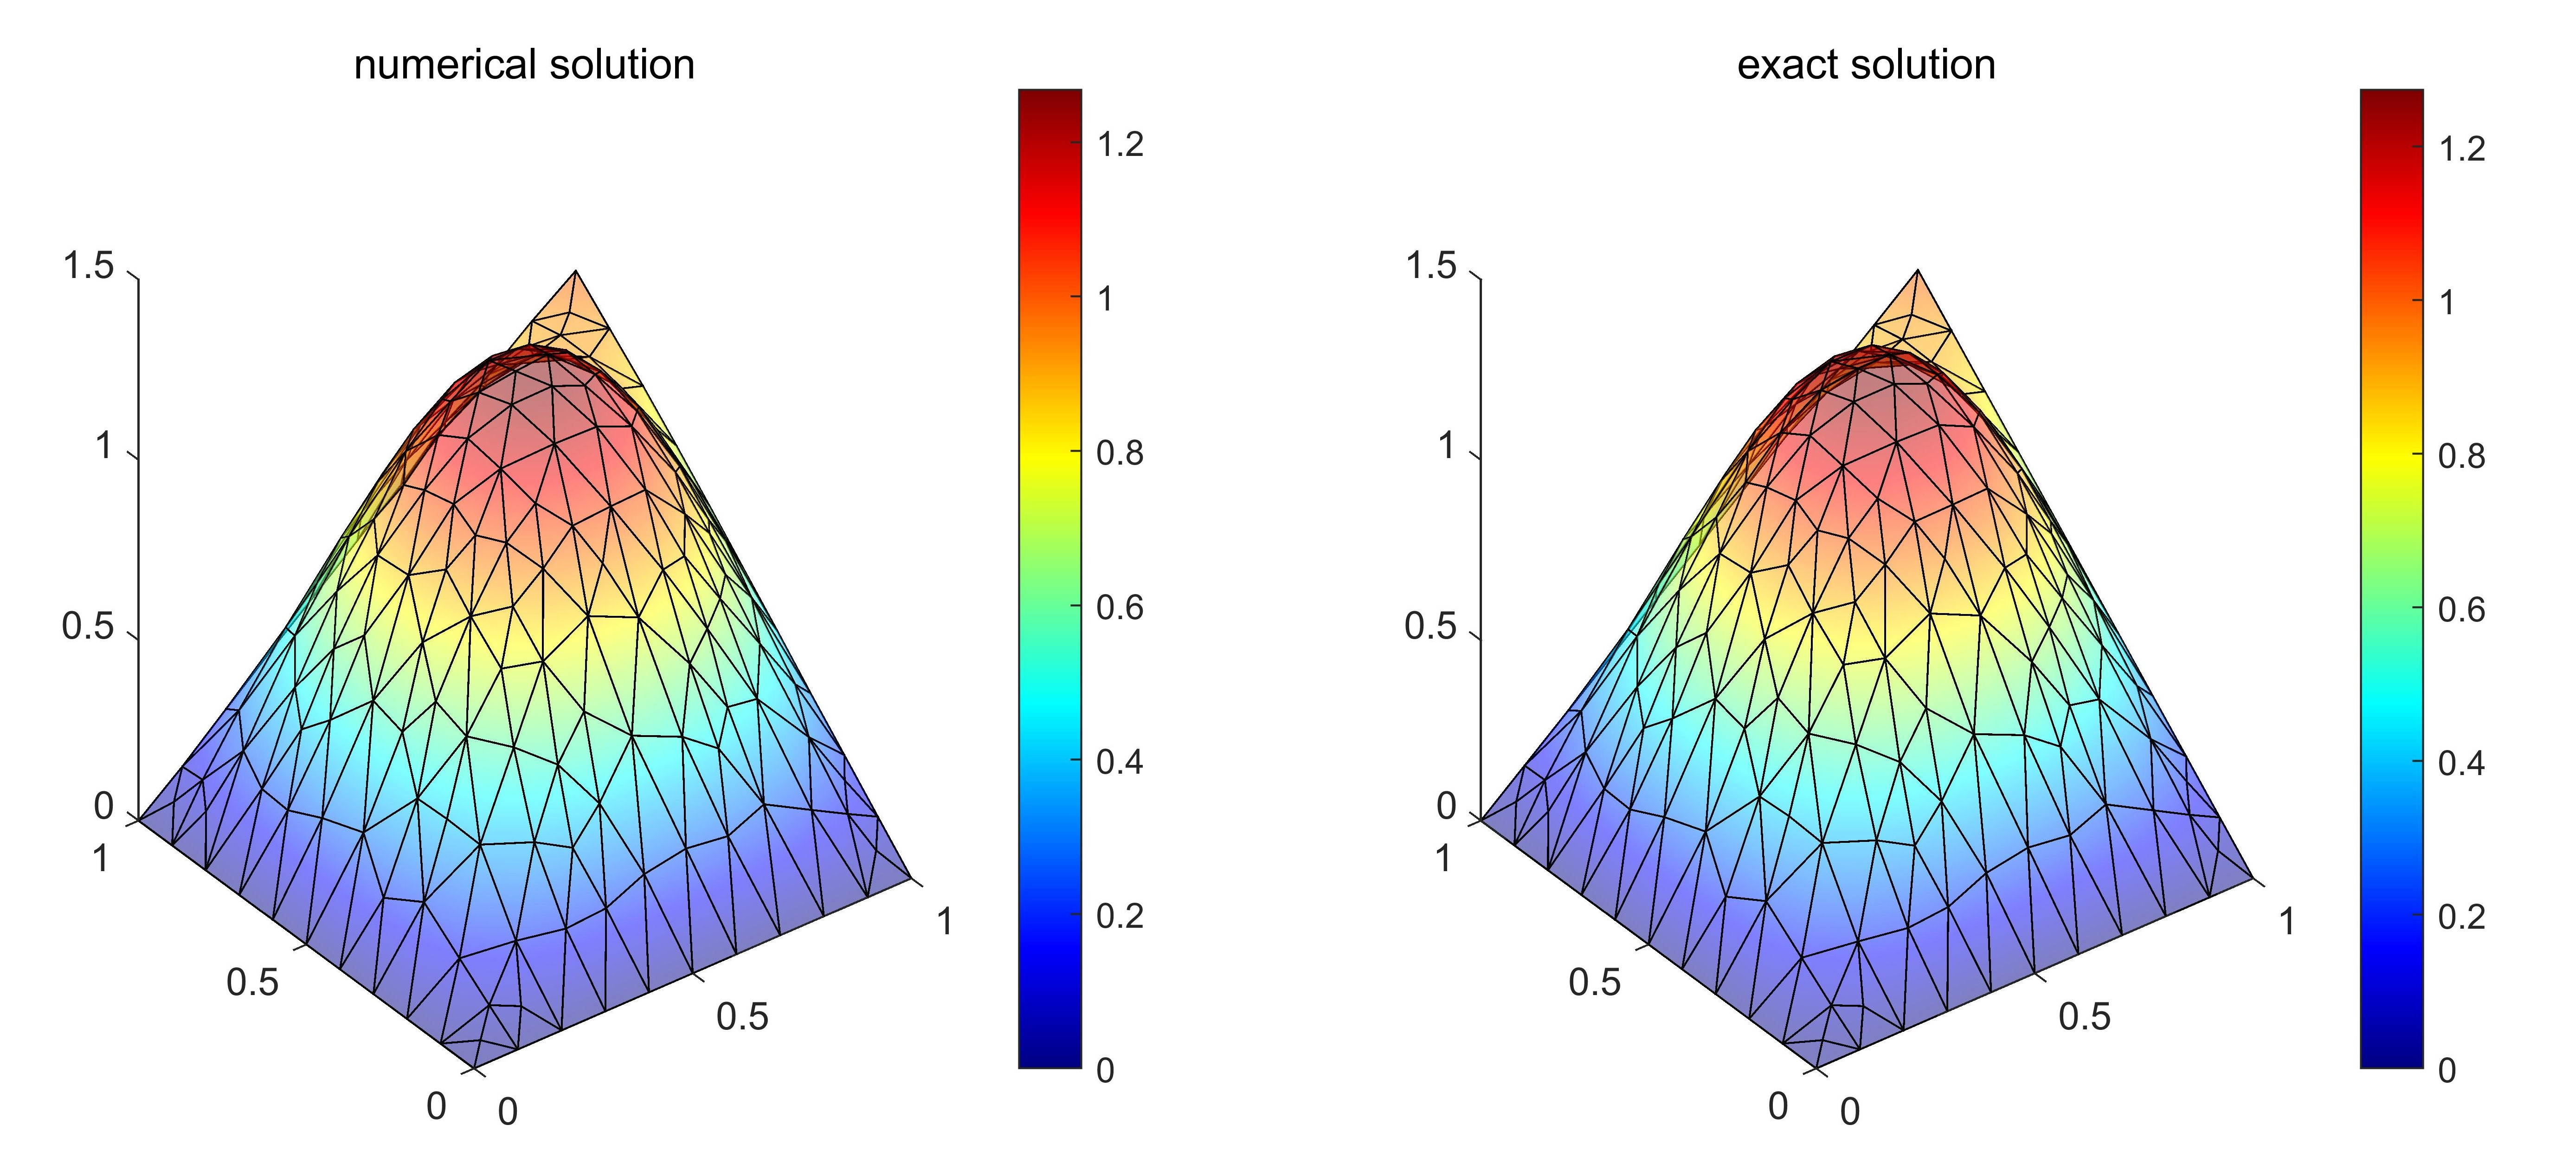
\includegraphics[width=\textwidth]{figure.jpg}
\end{figure}

\subsection{误差和收敛阶}
取剖分数$N=5n(1\le n\le 10),$分别计算$L^2$误差和$H^1$误差.需要注意的是横轴代表的含义
是"自由度",可以近似的认为是节点数量.所以有些图像看起来并不均匀.很奇怪的一点是这次误差
的收敛阶并没有像之前一样渐进收敛到$1$和$2$,而是在上下震荡,目前不清楚原因.
\begin{figure}[h]
	\centering
	  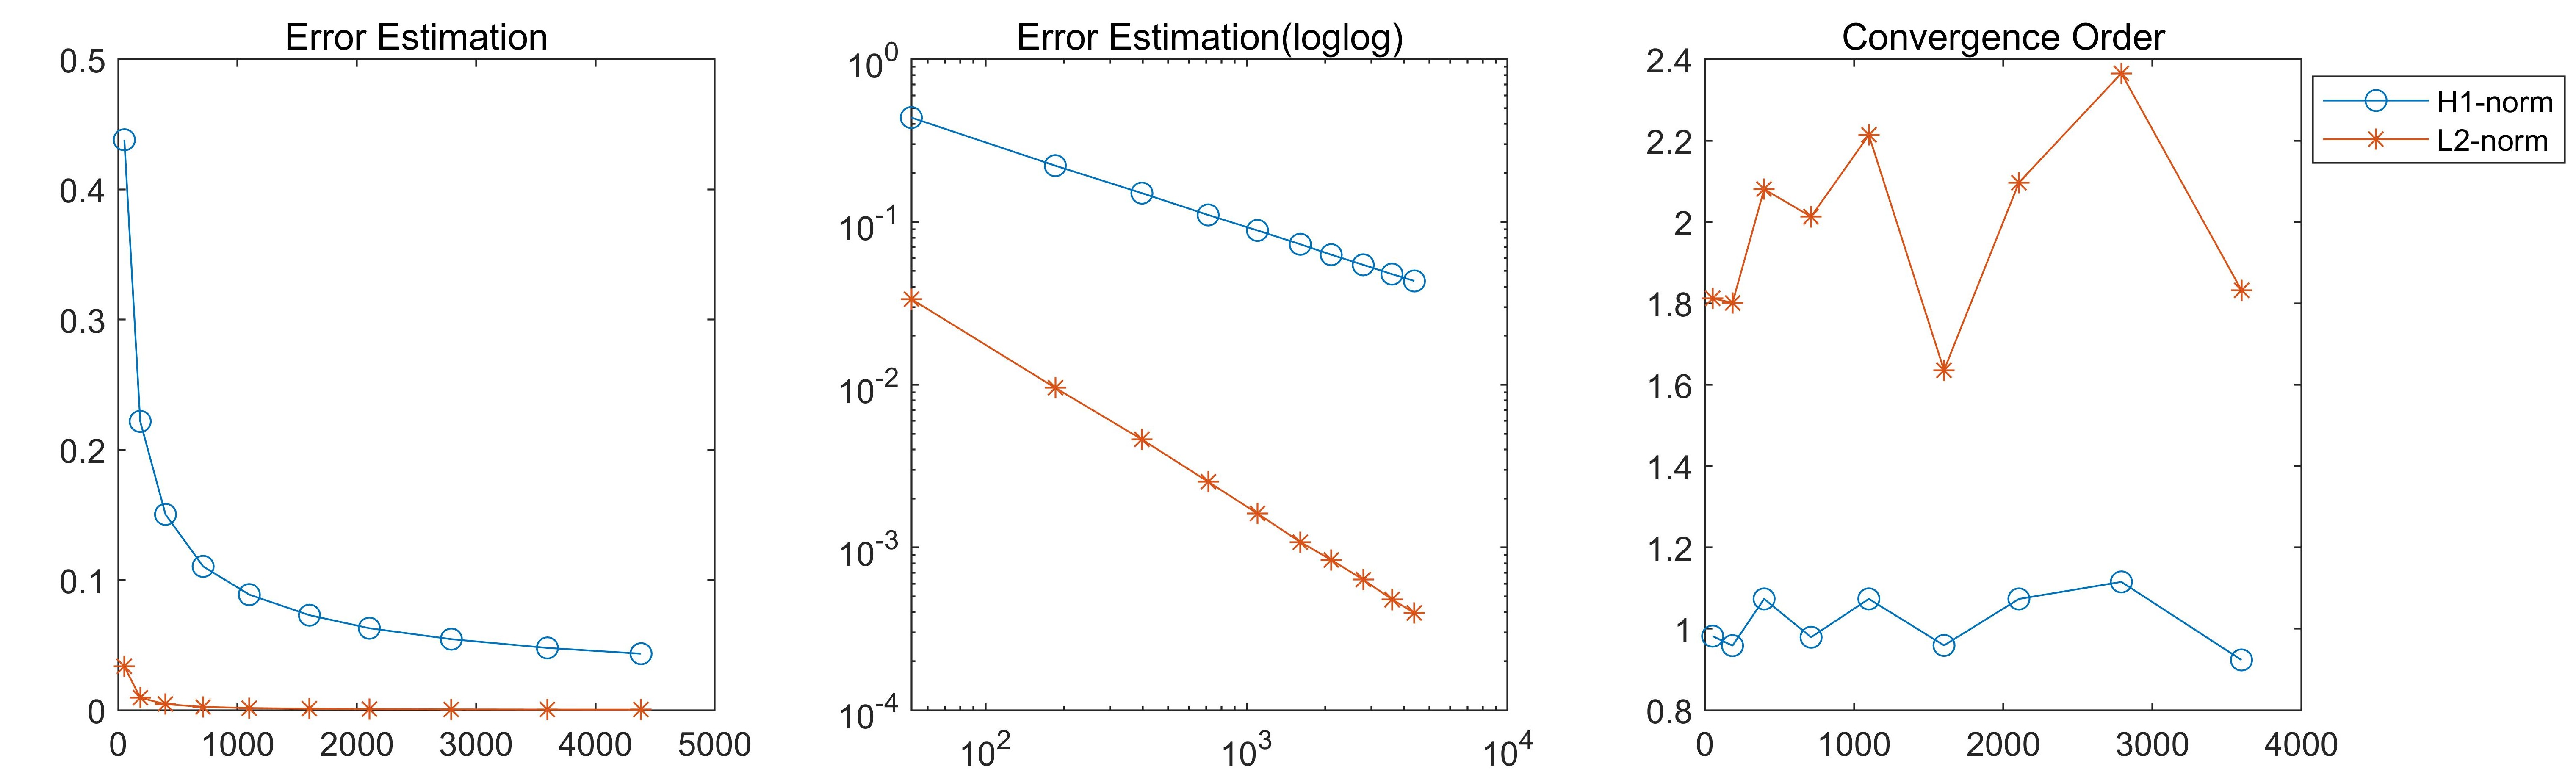
\includegraphics[width=\textwidth]{Order.jpg}
\end{figure}



\end{document}
